\documentclass[12pt]{article}

\usepackage{sbc-template}
\usepackage[brazil,american]{babel}
\usepackage[utf8]{inputenc}

\usepackage{graphicx}
\usepackage{url}
\usepackage{float}
\usepackage{listings}
\usepackage{color}
\usepackage{todonotes}
\usepackage{algorithmic}
\usepackage{algorithm}
\usepackage{hyperref}
\usepackage{indentfirst}
\usepackage[inline]{enumitem}

\graphicspath{{./images/}}

\sloppy

\title{Laboratório 2\\- ULA e FPULA –}

\author{GRUPO 6\\
	Dayanne Fernandes da Cunha, 13/0107191\\
	Lucas Mafra Chagas, 12/0126443\\
	Marcelo Giordano Martins Costa de Oliveira, 12/0037301\\
	Lucas Junior Ribas, 16/0052289\\
	Caio Nunes de Alencar Osório, 16/0115132\\
	Diego Vaz Fernandes, 16/0117925}

\address{Dep. Ciência da Computação -- Universidade de Brasília (UnB)\\
  CiC 116394 - OAC - Turma A
  \email{}
}

\begin{document}
\maketitle

\section{Objetivos}
\label{sec:Objetivos}

\begin{itemize}
\item Introduzir ao aluno a Linguagem de Descrição de \textit{Hardware Verilog};
\item Familiarizar o aluno com a plataforma de desenvolvimento \textit{FPGA DE2} da \textit{Altera} e o \textit{software QUARTUS-II};
\item Desenvolver a capacidade de análise e síntese de sistemas digitais usando \textit{HDL}.
\end{itemize}

\section{Ferramentas}
\label{sec:Materiais}

\begin{itemize}
\item FPGA DE2 da Altera 
\item QUARTUS-II
\item Verilog
\item HDL
\end{itemize}

\section{Exercícios}
\label{sec:exercicios}

Todos os códigos escritos neste laboratório podem ser encontrados no repositório \url{https://github.com/Dayof/OAC172} do \textit{GitHub}.

\subsection{Exercício 1. Implementação de um \textit{driver} para \textit{display} de 7 segmentos}
\label{subsec:1driver}

Conforme descrito no arquivo \textit{QuartusIIv3.txt} e \textit{Set.txt}, um novo projeto foi criado no diretório \textit{Lab2}, denominado \textit{Display}. 

Para as versões síncrona e assíncrona foram geradas as simulações temporais (Figura~\ref{fig:ex1st} e Figura~\ref{fig:ex1ast}) e funcionais (Figura~\ref{fig:ex1sf} e Figura~\ref{fig:ex1asf}).

\begin{figure}[H]
	\centering
	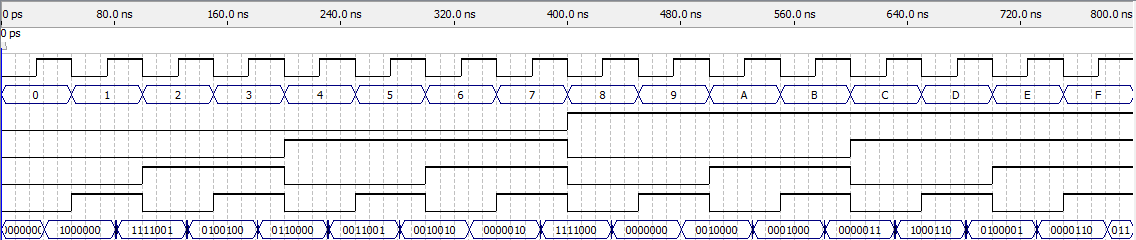
\includegraphics[width=.8\textwidth]{ex1_st.png}
	\caption{Simulação síncrona temporal do \textit{decoder7}.}
	\label{fig:ex1st}
\end{figure}

\begin{figure}[H]
	\centering
	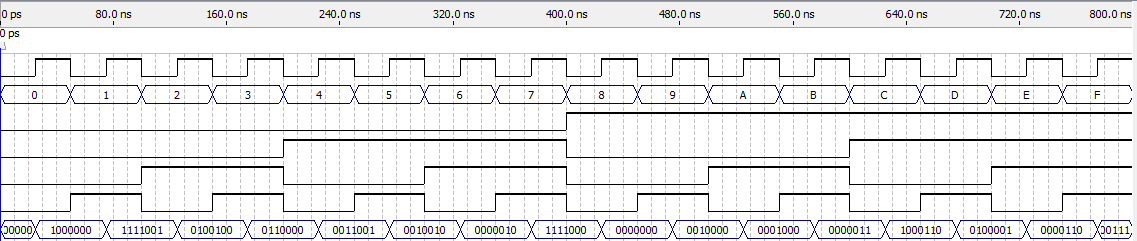
\includegraphics[width=.8\textwidth]{ex1_sf.png}
	\caption{Simulação síncrona funcional do \textit{decoder7}.}
	\label{fig:ex1sf}
\end{figure}

\begin{figure}[H]
	\centering
	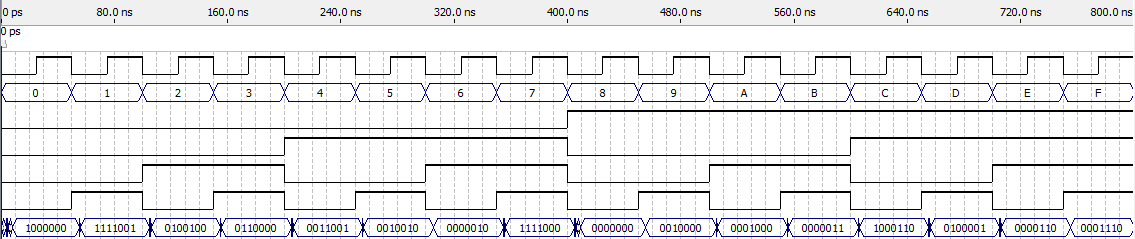
\includegraphics[width=.8\textwidth]{ex1_ast.png}
	\caption{Simulação assíncrona temporal do \textit{decoder7}.}
	\label{fig:ex1ast}
\end{figure}

\begin{figure}[H]
	\centering
	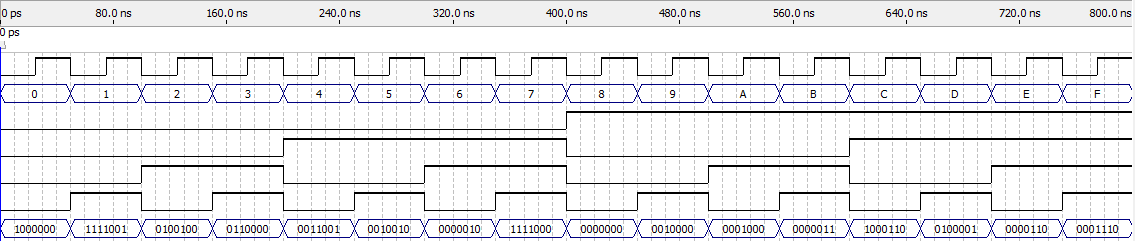
\includegraphics[width=.8\textwidth]{ex1_asf.png}
	\caption{Simulação assíncrona funcional do \textit{decoder7}.}
	\label{fig:ex1asf}
\end{figure}

Os requisitos físicos do \textit{decoder7} do \textit{driver} para \textit{display} de 7 segmentos foram analisados nas versões síncrona e assíncrona como é possível ver na Tabela~\ref{tab:req1}.

% max freq f=1/T
% max delay T=1/f

\begin{table}[H]
	\centering
	\begin{tabular}{|c|c|c|c|}
		\hline
		& \textbf{Elementos} & \textbf{Maior} & \textbf{Frequência máxima} \\
		& \textbf{lógicos} & \textbf{atraso (ns)} & \textbf{de operação (MHz)} \\\hline
		\hline
		\textbf{Síncrono} & 7 & ? & ? \\\hline
		\textbf{Assíncrono} & 7 & 9.761 & ? \\\hline
	\end{tabular}
	\caption{Requisitos físicos do \textit{display} de 7 segmentos assíncrono e síncrono.}
	\label{tab:req1}
\end{table}

O arquivo de interface \textit{TopDE.v} foi incluso no projeto, sintetizado e testado como é mostrado no link \url{https://youtu.be/wGKjze5PkcU}.

\subsection{Exercício 2. Unidade Lógica Aritmética de Inteiros}
\label{subsec:ulaint}

\subsubsection{ULA MIPS32}
\label{subsubsec:ulamips32}

% diagrama em blocos
% funções
% tabela verdade de cada operação

\subsubsection{Operações}
\label{subsubsec:2op}

% simulação temporal de cada operação
% usar valores comuns que gerem valores singulares (overflow, zero)

\subsubsection{Requisitos físicos}
\label{subsubsec:ulafis}

% para a ULA total e para cada operação
% número de elementos lógicos
% tempos de atraso
% máxima frequência de clock utilizável

\begin{table}[H]
	\centering
	\begin{tabular}{|c|c|c|c|}
		\hline
		& \textbf{Elementos} & \textbf{Tempo de} & \textbf{Frequência máxima de} \\
		& \textbf{lógicos} & \textbf{atraso (ns)} & \textbf{\textit{clock} utilizável (MHz)} \\
		\hline
		\textbf{ULA} & ? & ? & ? \\\hline
		\textbf{OPAND} & ? & ? & ? \\\hline
		\textbf{OPOR} & ? & ? & ? \\\hline
		\textbf{OPADD} & ? & ? & ? \\\hline
		\textbf{OPMFHI} & ? & ? & ? \\\hline
		\textbf{OPSLL} & ? & ? & ? \\\hline
		\textbf{OPMFLO} & ? & ? & ? \\\hline
		\textbf{OPSUB} & ? & ? & ? \\\hline
		\textbf{OPSLT} & ? & ? & ? \\\hline
		\textbf{OPSGT} & ? & ? & ? \\\hline
		\textbf{OPSRL} & ? & ? & ? \\\hline
		\textbf{OPSRA} & ? & ? & ? \\\hline
		\textbf{OPXOR} & ? & ? & ? \\\hline
		\textbf{OPSLTU} & ? & ? & ? \\\hline
		\textbf{OPNOR} & ? & ? & ? \\\hline
		\textbf{OPLUI} & ? & ? & ? \\\hline
		\textbf{OPSLLV} & ? & ? & ? \\\hline
		\textbf{OPSRAV} & ? & ? & ? \\\hline
		\textbf{OPSRLV} & ? & ? & ? \\\hline
		\textbf{OPMULT} & ? & ? & ? \\\hline
		\textbf{OPDIV} & ? & ? & ? \\\hline
		\textbf{OPDEBUG} & ? & ? & ? \\\hline
		\textbf{OPMULTU} & ? & ? & ? \\\hline
		\textbf{OPDIVU} & ? & ? & ? \\\hline
		\textbf{OPMTHI} & ? & ? & ? \\\hline
		\textbf{OPMTLO} & ? & ? & ? \\\hline
		\textbf{OPMADD} & ? & ? & ? \\\hline
		\textbf{OPMADDU} & ? & ? & ? \\\hline
		\textbf{OPMSUB} & ? & ? & ? \\\hline
		\textbf{OPMSUBU}  & ? & ? & ? \\\hline
	\end{tabular}
	\caption{Requisitos físicos da \textit{ULA} total e de cada operação.}
	\label{tab:req2}
\end{table}

\subsubsection{Funcionamento}
\label{subsubsec:ulafunc}

O projeto da \textit{ULA} de inteiros foi sintetizado utilizando a interface \textit{TopDE.v} na placa \textit{DE2-70} e seu funcionamento pode ser visto através do \textit{link} \url{?}. 

\subsection{Exercício 3. Unidade Aritmética de Ponto Flutuante }
\label{subsec:ulafloat}

\subsubsection{FPULA MIPS}
\label{subsubsec:fpulamips}

% diagrama em blocos
% funções (megawizard plug-in manager edit)
% tabela verdade de cada operação

\subsubsection{Operações}
\label{subsubsec:3op}

% simulação temporal de cada operação
% usar valores comuns que gerem valores singulares (overflow, underflow, NaN, zero)

\subsubsection{Requisitos físicos}
\label{subsubsec:fpulafis}

% para a FPULA total e para cada operação
% número de elementos lógicos
% número de ciclos para a conclusão da operação (tempos)
% máxima frequência de clock utilizável

\begin{table}[H]
	\centering
	\begin{tabular}{|c|c|c|c|}
		\hline
		& \textbf{Elementos} & \textbf{Número de ciclos} & \textbf{Frequência máxima de} \\
		& \textbf{lógicos} & \textbf{mínimo da operação (ns)} & \textbf{\textit{clock} utilizável (MHz)} \\
		\hline
		\textbf{FPULA} & ? & ? & ? \\\hline
		\textbf{OPADDS} & ? & ? & ? \\\hline
		\textbf{OPSUBS} & ? & ? & ? \\\hline
		\textbf{OPMULS} & ? & ? & ? \\\hline
		\textbf{OPDIVS} & ? & ? & ? \\\hline
		\textbf{OPSQRT} & ? & ? & ? \\\hline
		\textbf{OPABS} & ? & ? & ? \\\hline
		\textbf{OPNEG} & ? & ? & ? \\\hline
		\textbf{OPCEQ} & ? & ? & ? \\\hline
		\textbf{OPCLT} & ? & ? & ? \\\hline
		\textbf{OPCLE} & ? & ? & ? \\\hline
		\textbf{OPCVTSW} & ? & ? & ? \\\hline
		\textbf{OPCVTWS} & ? & ? & ? \\\hline
	\end{tabular}
	\caption{Requisitos físicos da \textit{FPULA} total e de cada operação.}
	\label{tab:req3}
\end{table}

\subsubsection{Funcionamento}
\label{subsubsec:fpulafunc}

O projeto da \textit{ULA} de ponto flutuante foi sintetizado utilizando a interface \textit{TopDE.v} na placa \textit{DE2-70} e seu funcionamento pode ser visto através do \textit{link} \url{?}. 

\bibliographystyle{sbc}
\bibliography{relatorio}

\end{document}
